\documentclass[conference]{IEEEtran}
\IEEEoverridecommandlockouts
% The preceding line is only needed to identify funding in the first footnote. If that is unneeded, please comment it out.
\usepackage{cite}
\usepackage{amsmath,amssymb,amsfonts}
\usepackage{algorithmic}
\usepackage{mathpazo}
\usepackage[spanish]{babel}
\usepackage[utf8]{inputenc}
\usepackage{graphicx}
\usepackage{textcomp}
\usepackage{xcolor}
%\usepackage{minted}
%\usemintedstyle{emacs}
\usepackage{url}
\usepackage{ctable}
\usepackage{float}
\usepackage{amsmath,amssymb,amsfonts}
\usepackage{makecell}
\usepackage{hyperref}
\usepackage{comment}
\hypersetup{
	colorlinks=true,
	linkcolor=blue,
	filecolor=magenta,      
	urlcolor=cyan,
}
\newcommand{\DNoise}{n_d}

\newcommand{\Est}[1]{\hat{#1}}
\newcommand{\Test}[1]{\expandafter\hat#1}

\def\BibTeX{{\rm B\kern-.05em{\sc i\kern-.025em b}\kern-.08em
    T\kern-.1667em\lower.7ex\hbox{E}\kern-.125emX}}
    
\begin{document}
\title{\bf{Trabajo final de curso de Fundamentos de la programación}}
%{\footnotesize \textsuperscript{*}}

\author{\IEEEauthorblockN{
Delgado, G. (60\%)}
\IEEEauthorblockA{\textit{Escuela de Ciencias de la Computación} \\
\textit{Universidad Nacional de Ingeniería}\\
Lima, Per\'u \\
\texttt{gustavo.delgado.r@uni.pe}}
\and
\IEEEauthorblockN{ 
Mori, J. (40\%)}
\IEEEauthorblockA{\textit{Escuela de Ciencias de la Computación} \\
\textit{Universidad Nacional de Ingeniería}\\
Lima, Perú \\
\texttt{jean.mori.m@uni.pe }}}

\maketitle

\begin{abstract}
El modelado del lenguaje se ha abordado recientemente utilizando m\'etodos de entrenamiento no supervisados como ELMo y BERT. Sin embargo, sigue siendo un desaf\'io equipar adecuadamente las redes neuronales con una dependencia a largo plazo. 

En efecto, pese a que los modelos secuencia a secuencia son bastante vers\'atiles y se utilizan en una variedad de tareas de NLP, una desventaja cr\'itica es el dise\~no vectorial del contexto de longitud fija que no puede recordar oraciones largas. Un enfoque para resolver el problema de la p\'erdida de informaci\'on relevante en oraciones largas es utilizar el mecanismo de atenci\'on que necesita calcular un valor para cada combinaci\'on de palabras de entrada y salida, por lo que suele ser costoso.  En  arquitecturas que utilizan el modelo Transformer, se utiliza variantes del mecanismo de atenci\'on  para aprender tambi\'en las dependencias de entrada y salida y pese al potencial de este algoritmo, tienen el problema de no extenderse m\'as all\'a de un cierto nivel debido al uso del contexto de longitud fija no puede modelar dependencias que son m\'as largas que una longitud fija.

Para resolver estos problemas se plantea un nuevo modelo llamado Transformer-XL, que forma parte  de un nuevo conjunto de t\'ecnicas utilizadas para entrenar modelos altamente eficientes y de alto rendimiento en NLP. 

En este trabajo se implementan sobre conjuntos reducidos como Penn Treebank varias de las t\'ecnicas recientes como el Transformer- XL, XLNet, que son una variante del  Transformer.

\vspace{0.2cm}


\'Indice de T\'erminos— RNN, modelos seq2seq, mecanismos de atenci\'on, transformers,  Hugging Face.
    
\end{abstract}

\section{Introducci\'on}
Una tendencia dada en el ICRL \footnote{International Conference on Learning Representations } y en el NAACL- HLT \footnote{Annual Conference of the North American Chapter of the Association for Computational Linguistics: Human Language Technologies.} celebrados en el 2019,  muestra que las  RNN tienen una mayor ca\'ida en publicaciones. Esto no es sorprendente porque, aunque los RNN son intuitivos para los datos secuenciales, sufren un inconveniente masivo: no pueden ser paralelizados y, por lo tanto, no pueden aprovechar el factor m\'as importante que ha impulsado el progreso en la investigaci\'on desde $2012$: la potencia de c\'alculo. Los RNN nunca han sido populares en visi\'on computacional y aprendizaje por refuerzo y para NLP, est\'an siendo reemplazados por arquitecturas basadas en la atenci\'on.

\begin{figure}[h]
	\centering
	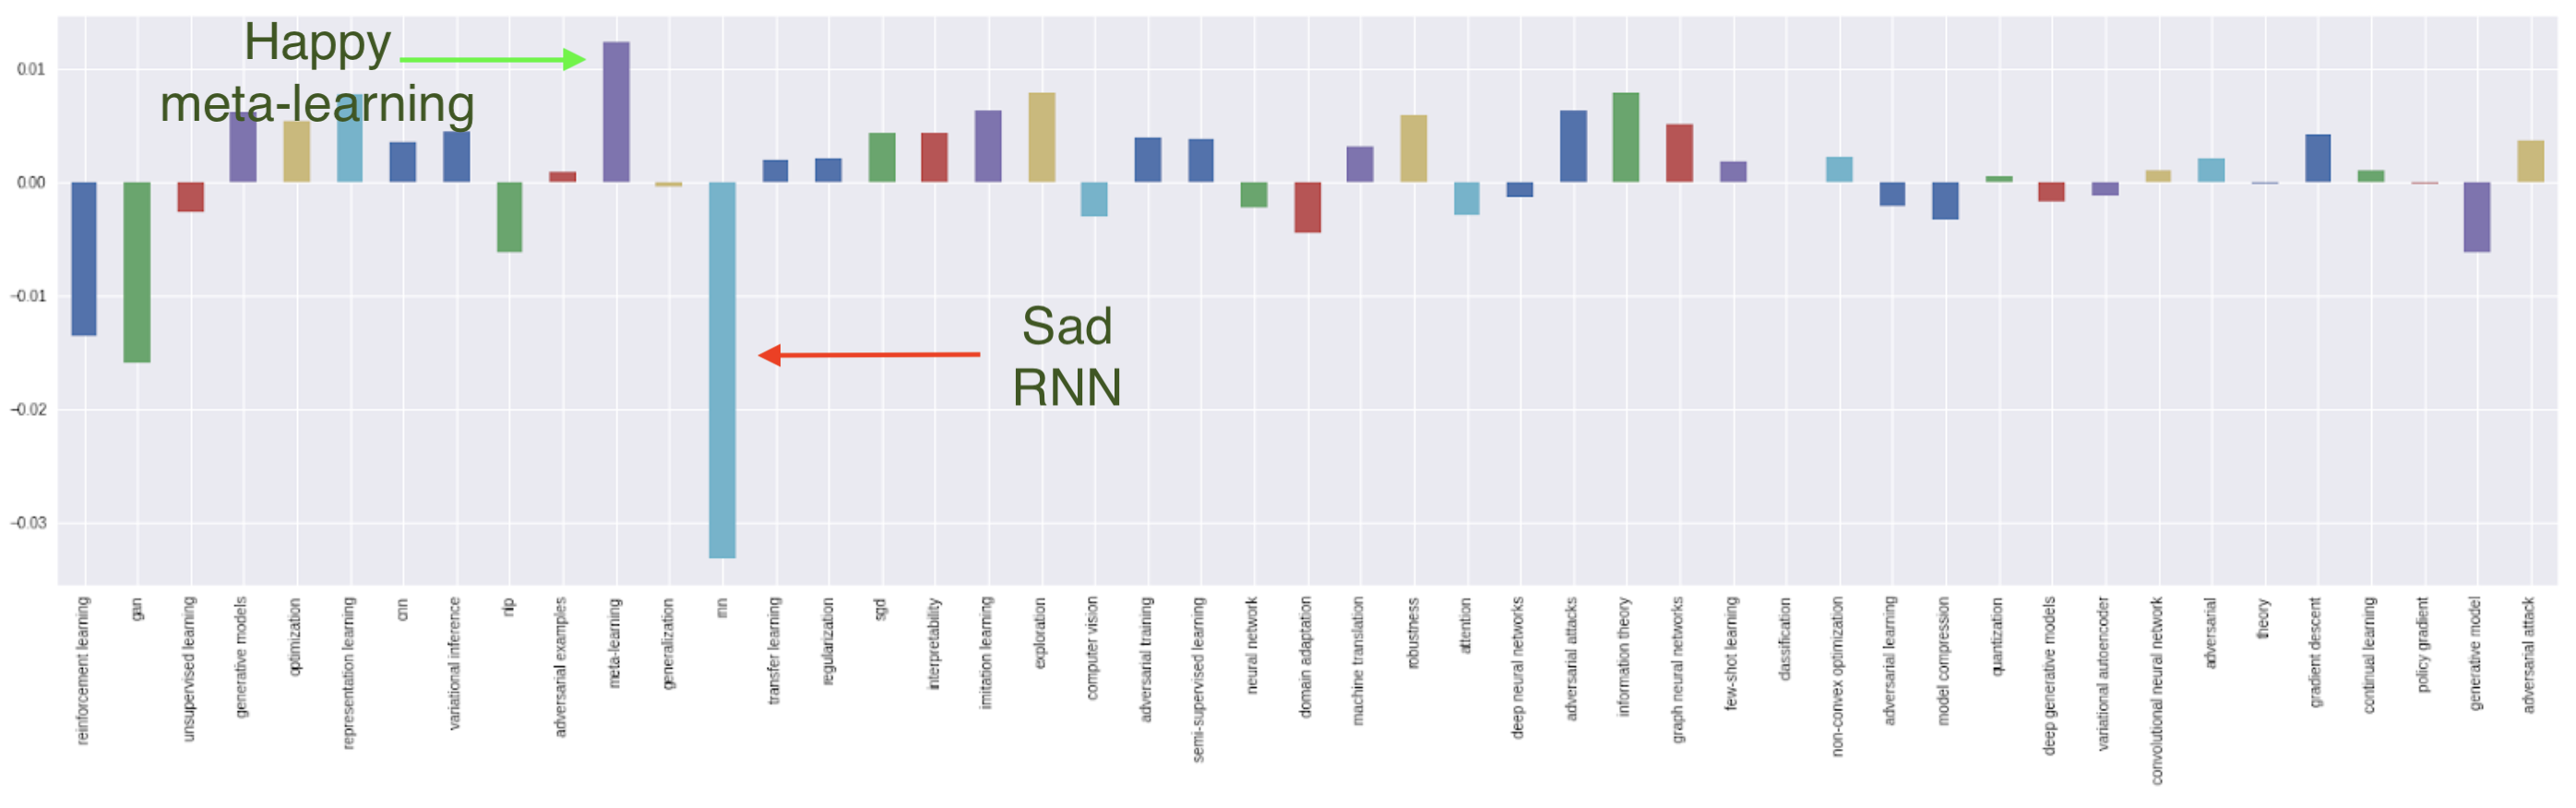
\includegraphics[scale=.2]{imagenes/rnn.png}
	\caption{Estadisticas de ICRL 2019} 
\end{figure}




\section{Marco Te\'orico}

\subsection{El modelo secuencia a secuencias}
El modelo secuencia a secuencia o seq2seq naci\'o en el campo del modelamiento del lenguaje \cite{b6} y tiene como objetivo transformar una secuencia de entrada, en una nueva secuencias, ambas de longitudes arbitrarias. Ejemplos que utilizan estos modelos  incluyen la traducci\'on autom\'atica entre varios lenguajes de texto o audio, generaci\'on de di\'alogos de preguntas y respuestas, correctores ortogr\'aficos o incluso analizar oraciones en \'arboles de gram\'atica.

\vspace{0.2cm}

El modelo seq2seq normalmente tiene una arquitectura encoder-decoder, compuesta de:

\begin{enumerate}
\item Un encoder procesa la secuencia de entrada y comprime la informaci\'on en un vector de contexto, de  longitud fija. Esta representaci\'on es resumen del significado de toda la secuencia de entrada.
\item Un decoder se inicializa con el vector de contexto para emitir una salida transformada. 

Tanto el encoder y decoder son redes neuronales recurrentes, es decir, que utilizan unidades LSTM \cite{b17, b18} o GRU \cite{b19}. 

\end{enumerate}

\vspace{0.2cm}

En \cite{b20}, se realiza una b\'usqueda entre diferentes arquitecturas RNN incluyendo el GRU en tareas como el modelamiento de lenguaje, recomendando agregar un sesgo de 1 a la puerta de olvido de cada LSTM en cada aplicaci\'on, lo que resultan en un mejor rendimiento.

\begin{figure}[h]
	\centering
	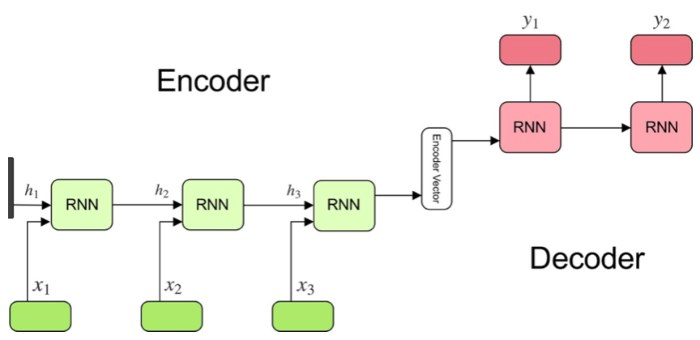
\includegraphics[scale=.3]{imagenes/seq2seq.jpg}
	\caption{Estructura de un modelo seq2seq} 
\end{figure}

\subsubsection{Problemas con los modelos seq2seq}

Pese a que los  modelos encoder-decoder son una subclase ampliamente utilizada tiene ciertos incovenientes:

\begin{itemize}
\item El c\'alculo secuencial evita la paralelizaci\'on.
	\item Comprime toda la informaci\'on de una oraci\'on de entrada en un vector de longitud fija que luego toma el decoder, lo que conduce a una disminuci\'on en el rendimiento cuando se trata de oraciones largas. 
\end{itemize}

El mecanismo de atenci\'on naci\'o propuesto por Bahdanau \cite{b2} apareci\'o para resolver algunos de estos problemas.

\subsection{Mecanismos de atenci\'on}

En estos modelos, cada vez que el modelo predice una palabra de salida, solo usa partes de una entrada donde se concentra la información m\'as relevante en lugar de una oraci\'on completa. El encoder funciona como de costumbre, pero el estado oculto del decoder se calcula con un vector de contexto, la salida anterior y el estado oculto anterior. Los vectores de contexto se calculan como una suma ponderada de anotaciones generadas por el encoder con un vector de contexto separado para cada palabra objetivo. 


Sean $\mathbf{x}$ una secuencia de entrada de longitud de $n$ y sea $\mathbf{y}$ una secuencia de longitud $m$ a generar:



\begin{align*}
	\mathbf{x} &= [x_1, x_2, \dots, x_n] \\
	\mathbf{y} &= [y_1, y_2, \dots, y_m]
\end{align*}

En el caso de un LSTM bidireccional, estas anotaciones son concatenaciones de estados ocultos en las direcciones hacia adelante $\overrightarrow{\boldsymbol{h}}_i$ y hacia atr\'as $\overleftarrow{\boldsymbol{h}}_i$. Una concatenaci\'on de dos representa el estado del encoder. La motivaci\'on es incluir tanto las palabras anteriores como las siguientes en la anotaci\'on de una palabra.

\[
\boldsymbol{h}_i = [\overrightarrow{\boldsymbol{h}}_i^\top; \overleftarrow{\boldsymbol{h}}_i^\top]^\top, i=1,\dots,n
\]


La red del decodificador tiene un estado oculto $\boldsymbol{s}_t=f(\boldsymbol{s}_{t-1}, y_{t-1}, \mathbf{c}_t)$, para la palabra de salida en la posici\'on $t=1,\dots,m$, donde el vector de contexto $\mathbf{c}_t$, es una suma de estados ocultos de la  secuencia de entrada, ponderada por puntajes de alineaci\'on:


\begin{align*}
	\mathbf{c}_t &= \sum_{i=1}^n \alpha_{t,i} \boldsymbol{h}_i \\
	\alpha_{t,i} &= \text{align}(y_t, x_i) \\
	&= \frac{\exp(\text{score}(\boldsymbol{s}_{t-1}, \boldsymbol{h}_i))}{\sum_{i'=1}^n \exp(\text{score}(\boldsymbol{s}_{t-1}, \boldsymbol{h}_{i'}))}.
\end{align*}


El modelo de alineaci\'on asigna una puntuaci\'on $\alpha_{t,i}$ al par de entrada en la posici\'on $i$ y salida en la posici\'on $t$, $(y_t, x_i)$, en funci\'on de qu\'e tan bien coinciden. El conjunto de $\{\alpha_{t, i}\}$ son pesos que definen cu\'anto de cada estado oculto de la fuente debe considerarse para cada salida.

\vspace{0.2cm}

En el art\'iculo de Bahdanau, el puntaje de alineaci\'on $\alpha$ est\'a parametrizado por una red  con una sola capa oculta y esta red se entrena conjuntamente con otras partes del modelo. Por lo tanto, la funci\'on de puntuaci\'on tiene la siguiente forma, dado que $\tanh$ se usa como una funci\'on de activaci\'on no lineal:

\[
\text{score}(\boldsymbol{s}_t, \boldsymbol{h}_i) = \mathbf{v}_a^\top \tanh(\mathbf{W}_a[\boldsymbol{s}_t; \boldsymbol{h}_i])
\]

donde ambos $\mathbf{v}_a$ y $\mathbf{W}_a$ son matrices de peso que se aprender\'an en el modelo de alineaci\'on.

La matriz de puntajes de alineaci\'on muestra expl\'icitamente la correlaci\'on entre las palabras de entrada y de salida.


\begin{figure}[h]
	\centering
	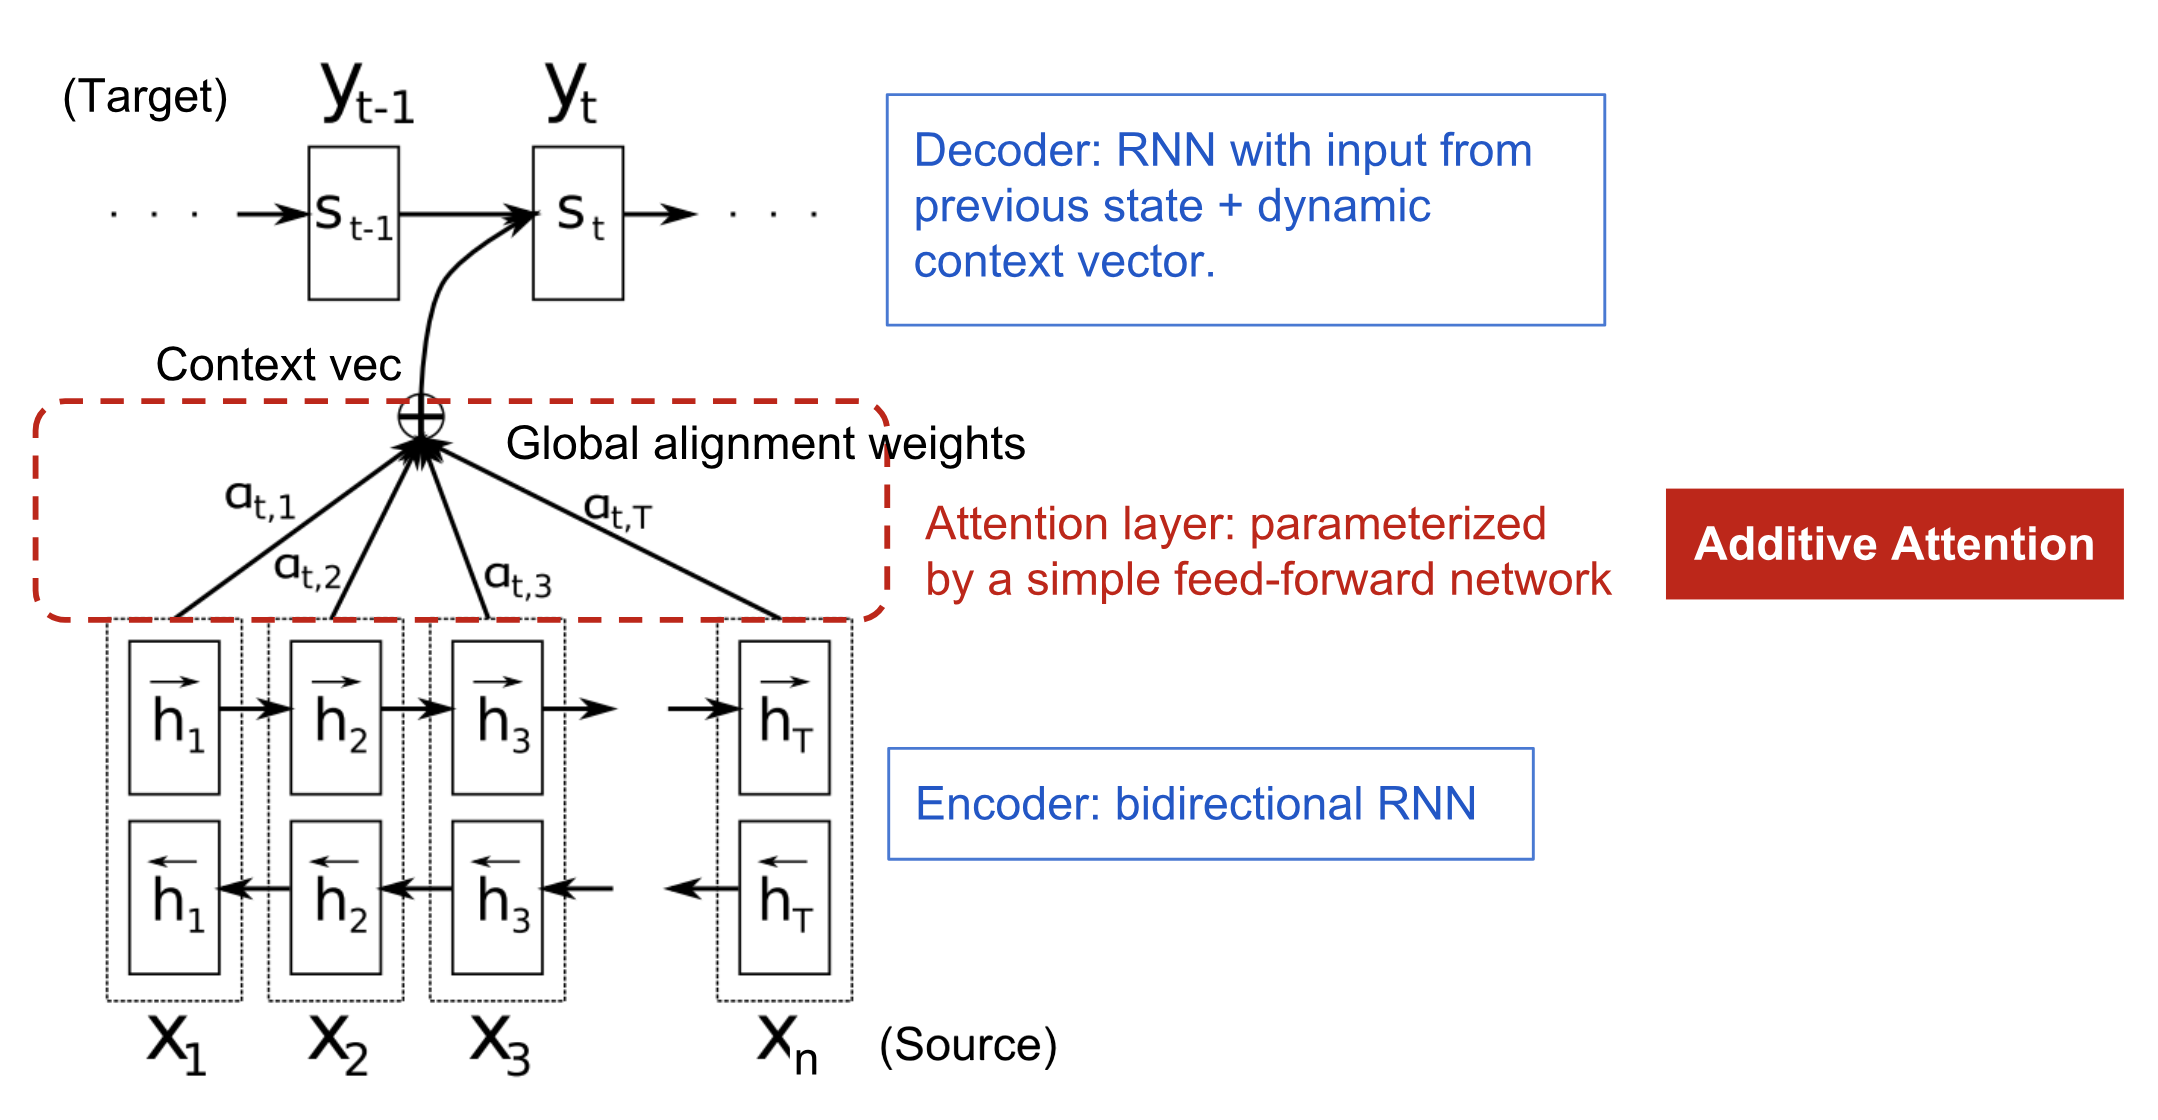
\includegraphics[scale=.28]{imagenes/encoder-decoder-attention.png}
	\caption{Modelo encoder-decoder con atenci\'on aditiva} 
\end{figure}

\subsection{Familia de mecanismo de atenci\'on}

Dada la gran mejora de la atenci\'on en la traduccio\'n autom\'atica, pronto se extendi\'o al campo de la visi\'on computacional \cite{b5} y la gente comenz\'o a explorar otras formas de mecanismos de atenci\'on \cite{b1, b4, b7}.  

A continuaci\'on se muestra una tabla resumen de varios mecanismos de atenci\'on populares y las correspondientes funciones de puntuación de alineaci\'on:

\begin{table}[!h]
\begin{tabular}{|c|c|c|}
\hline
Nombre            & Alignment score funci\'on                                                                                                                                                                                                                   & Paper                      \\ \hline
\begin{tabular}[c]{@{}c@{}}Content-base\\  attention \\ \end{tabular} & $\text{score}(\textbf{s}_t, \textbf{h}_i) = \text{cosine}[\textbf{s}_t, \textbf{h}_i]$                                                                                                                                                                                       & \textbf{Graves 2014}\cite{b3} \\ \hline
		Additive(*)  &$\text{score}(\textbf{s}_t, \textbf{h}_i) = \textbf{v}_a^{T}\tanh[\textbf{s}_t, \textbf{h}_i]$  
		                                                                                                                                                                             & \textbf{Bahdanau 2015 }\cite{b2}\\ \hline
		Location(**)  & \begin{tabular}[c]{@{}c@{}}$\alpha_{t,i} = \text{softmax}(\textbf{W}_a\textbf{s}_t)$\\ \end{tabular}  & \textbf{Luong 2015}\cite{b4} \\ \hline
		General(***)  & $\text{score}(\textbf{s}_t, \textbf{h}_i) = \textbf{s}_t^{T}\textbf{W}_a\textbf{h}_i$                                                                                                                                                                                                                    & \textbf{Luong 2015}\cite{b4}    \\ \hline
		Dot-Product & $\text{score}(\textbf{s}_t, \textbf{h}_i) = \textbf{s}_t^T\textbf{h}_i$                                                                                                                                                                                                                      &  \textbf{Luong 2015}\cite{b4}  \\ \hline
		\begin{tabular}[c]{@{}c@{}}Scaled Dot-\\ Product (****)\end{tabular}   & \begin{tabular}[c]{@{}c@{}}$\text{score}(\textbf{s}_t, \textbf{h}_i) = \frac{ \textbf{s}_t^T\textbf{h}_i}{\sqrt{n}}$\\ \end{tabular} &\textbf{Waswani 2017}\cite{b1}\\ \hline
	\end{tabular}
\end{table}

\begin{itemize}
\item \scriptsize{(*) Conocido como \texttt{concat} en Luong\cite{b4} y como \texttt{additive attention} en Vaswani \cite{b1}}.
\item (**) La ecuaci\'on simplifica la alineaci\'on softmax para que solo dependa de la posici\'on del objetivo.
\item (***) $\textbf{W}_a$ es una matriz de pesos entrenables en la capa de atenci\'on.
\item (****) Se agrega un factor de escala $1/\sqrt{n}$, motivada por la preocupaci\'on cuando la entrada es grande, el softmax puede tener un gradiente extremadamente peque\~no, dif\'icil para un aprendizaje eficiente.
	
\end{itemize}

\vspace{0.2cm}


Aqu\'i hay un resumen de categor\'ias m\'as amplias de mecanismos de atenci\'on:

\begin{table}[!h]
	\begin{tabular}{|l|l|l|}
		\hline
		\multicolumn{1}{|c|}{\textbf{Nombre}} & \multicolumn{1}{c|}{\textbf{Definici\'on}}                                                                                                                                                                                           & \multicolumn{1}{c|}{\textbf{Papers}} \\ \hline
		Global                                & \begin{tabular}[c]{@{}l@{}}Utiliza todos los estados ocultos\\ del encoder para calcular \\ el vector de contexto.\end{tabular}                                                                                                     &\textbf{Xu 2015}\cite{b7}           \\ \hline
		Local                                 & \begin{tabular}[c]{@{}l@{}}Elige una posici\'on en la oraci\'on \\ de entrada para determinar la\\ ventana de palabras a considerar.\end{tabular}                                                                                      &\textbf{Luong 2016} \cite{b6}
		       \\ \hline
		Auto-atencion                         & \begin{tabular}[c]{@{}l@{}}Relaciona diferentes posiciones\\ de una sola secuencia para\\ calcular su representaci\'on\\ interna\end{tabular}                                                                                        &\textbf{Cheng 2017} \cite{b13}          \\ \hline
		Bidireccional                         & \begin{tabular}[c]{@{}l@{}}El modelo atiende la hip\'otesis \\ y la premisa y ambas \\ representaciones se concatenan\end{tabular}                                                                                                   &\textbf{Seo 2017} \cite{b14}          \\ \hline
		Clave-Valor                           & \begin{tabular}[c]{@{}l@{}}Los vectores de salida se separan \\ en claves para calcular la atenci\'on \\ y los valores para codificar la\\ distribuci\'on de la  siguiente\\ palabra y la representacion \\ del contexto.\end{tabular} & \textbf{Mino 2017}\cite{b15}          \\ \hline
		Jerarqu\'ia Anidada                     & \begin{tabular}[c]{@{}l@{}}Dos niveles de atenci\'on: primero\\ a nivel de palabra  y segundo a\\  nivel de oraci\'on.\end{tabular}                                                                                                    & \textbf{Yang 2016}\cite{b16}          \\ \hline
	\end{tabular}
\end{table}

\subsubsection{Auto-atenci\'on}

La auto-atenci\'on es un mecanismo de atenci\'on que relaciona diferentes posiciones de una sola secuencia para calcular una representaci\'on de la misma secuencia. 



\subsection{Transformers}

El modelo Transformer, propuesto en el paper \textcolor{orange}{Attention Is All You Need}, se basa en la auto-atenci\'on sin el uso de RNN. Como resultado, es altamente paralelo y requiere menos tiempo para entrenar, al tiempo que establece resultados de vanguardia en modelamiento de lenguaje y la traducci\'on autom\'atica.

El Transformer se basa en una estructura encoder-decoder. La diferencia entre este y cualquier otro modelo es que el Transformer se basa completamente en mecanismos de atenci\'on y capas puntuales totalmente conectadas tanto para el encoder como para el decoder. 


El componente principal en el Transformer es la unidad de mecanismo de auto-atenci\'on de m\'ultiples cabeceras. El transformador ve la representaci\'on codificada de la entrada como un conjunto de pares clave-valor (K, V), ambos de dimensi\'on $n$ (longitud de secuencia de entrada). En el contexto de NMT, tanto las claves como los valores son estados ocultos del encoder. En el decoder, la salida anterior se comprime en una consulta (Q de dimensi\'on $m$) y la siguiente salida se produce al mapear esta consulta y el conjunto de claves y valores.

\vspace{0.2cm}

El transformador adopta la atenci\'on escalada del producto punto: la salida es una suma ponderada de los valores, donde el peso asignado a cada valor est\'a determinado por el producto punto de la consulta con todas las claves:

\[
\text{Attention}(\mathbf{Q}, \mathbf{K}, \mathbf{V}) = \text{softmax}(\frac{\mathbf{Q}\mathbf{K}^\top}{\sqrt{n}})\mathbf{V}
\]


En lugar de solo calcular la atenci\'on una vez, el mecanismo de m\'ultiples cabeceras corre la atenci\'on escalada del producto puntos varias veces en paralelo. Las salidas de atenci\'on independientes simplemente se concatenan y se transforman linealmente en las dimensiones esperadas.

\begin{align*}
\text{MultiHead}(\mathbf{Q}, \mathbf{K}, \mathbf{V}) &= [\text{head}_1; \dots; \text{head}_h]\mathbf{W}^O \\
\text{donde head}_i &= \text{Attention}(\mathbf{Q}\mathbf{W}^Q_i, \mathbf{K}\mathbf{W}^K_i, \mathbf{V}\mathbf{W}^V_i)
\end{align*}

donde $\mathbf{W}^Q_i$, $\mathbf{W}^K_i$, $\mathbf{W}^V_i$ y $\mathbf{W}^O$ son matrices de par\'ametros para aprender.


\begin{figure}[h]
	\centering
	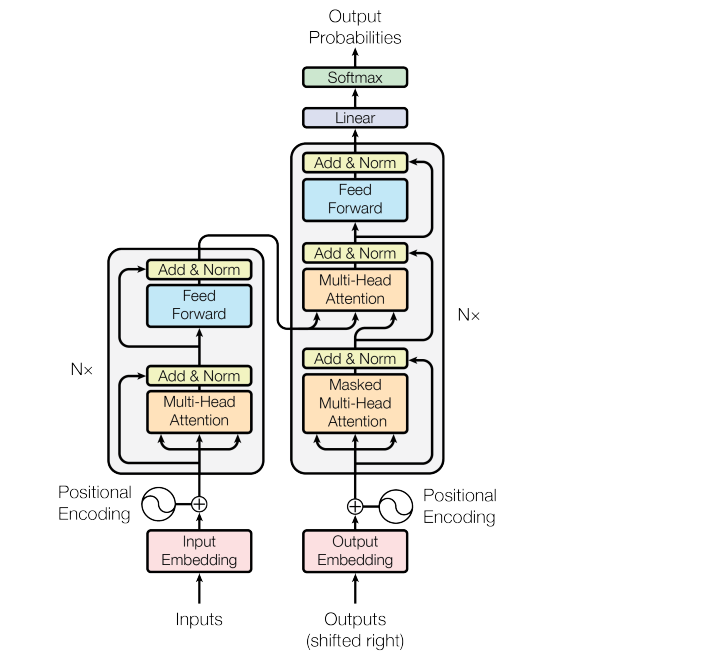
\includegraphics[scale=.12]{imagenes/transformer.png}
	\caption{Arquitectura del Transformer} 
\end{figure}
\subsubsection{Limitaciones del transformer}
El transformer es una mejora con respecto a los modelos seq2seq basados en RNN. Pero tiene algunas limitaciones:

\begin{itemize}
\item La atenci\'on solo puede ocuparse de cadenas de texto de longitud fija. El texto debe dividirse en un cierto n\'umero de segmentos  antes de ser alimentado al sistema como entrada.
\item Esta segmentaci\'on del texto provoca la fragmentaci\'on del contexto \footnote{context fragmentation}. Por ejemplo, si una oraci\'on se divide en dos, se pierde una cantidad significativa de contexto. En otras palabras, el texto se divide sin considerar la oraci\'on o cualquier otro l\'imite sem\'antico.
\end{itemize}


\section{Estado del Arte}
La arquitectura del transformador ya ha dado un paso adelante en 2019 con la publicaci\'on del transformer-xl \cite{b25} y otras arquitecturas relacionadas \cite{b24, b25, b26, b27, b28, b29}. 


\subsection{Transformador Universal}

El Transformador Universal es un modelo de secuencia recurrente auto-atento en paralelo en el tiempo, que es paralelizable sobre la secuencia de entrada. Al igual que el transformador base, tiene un  \texttt{campo receptivo global} (lo que significa que mira muchas palabras a la vez). La idea nueva y principal es que en cada paso recurrente, el transformador universal refina iterativamente sus representaciones para todos los s\'imbolos de la secuencia utilizando la auto-atenci\'on seguida de una funci\'on de transici\'on compartida en todas las posiciones y pasos de tiempo.

\vspace{0.2cm}

El Universal Transformer, combina el modelo original Transformer con una t\'ecnica llamada \textcolor{green}{Adaptive Computation Time}, un mecanismo que permite la aplicaci\'on del encoder un n\'umero variable de veces y la aplicaci\'on del decoder un n\'umero variable de veces.


El objetivo de Universal Transformer es lograr un buen rendimiento tanto en traducci\'on de lenguaje como en tareas algor\'itmicas con un solo modelo. Los autores del Universal Transformer se\~nalan que es un modelo completo de Turing.


\subsection{BERT}

BERT fue uno de los primeros modelos que muestra que los transformadores pueden alcanzar el rendimiento a nivel humano en una variedad de tareas basadas en el lenguaje: responder preguntas, clasificar sentimientos o clasificar si dos oraciones se suceden naturalmente.

\vspace{0.2cm}

BERT consiste en una simple pila de bloques transformadores. Esta pila est\'a pre-entrenada en un gran corpus de dominio general que consta de $800$ millones de palabras de libros en ingl\'es y $2.5$ mil palabras de texto de art\'iculos de Wikipedia en ingl\'es sin marcado y utiliza la tokenizaci\'on WordPiece, que se encuentra entre las secuencias de nivel de palabra y nivel caracter.


BERT utiliza la tokenizaci\'on de WordPiece, que se encuentra entre las secuencias de nivel de palabra y de nivel de palabra. Este divide palabras como \textcolor{orange}{walking} en los tokens \textcolor{blue}{walk}  y \textcolor{blue}{\#\# ing}. Esto permite que el modelo haga algunas inferencias basadas en la estructura de las palabras: dos verbos que terminan en \textcolor{green}{-ing} tienen funciones gramaticales similares, y dos verbos que comienzan con \textcolor{green}{walk} tienen una funci\'on sem\'antica similar.

\vspace{0.2cm}

En un experimento de ablaci\'on, los autores muestran que la mayor mejora en comparaci\'on con los modelos anteriores proviene de la naturaleza bidireccional del BERT. Es decir, modelos anteriores como GPT usaban una m\'ascara autoregresiva, que solo permit\'ia atenci\'on sobre los tokens anteriores. El hecho de que en BERT toda la atenci\'on se centre en toda la secuencia es la causa principal del rendimiento mejorado. Es por eso que la \textbf{B} en BERT significa \textcolor{red}{bidireccional}.


El modelo BERT m\'as grande utiliza $24$ bloques de transformadores, una dimensi\'on de integraci\'on de $1024$ y $16$ cabeceras de atenci\'on, lo que da como resultado par\'ametros de $340M$.


\subsection{GPT-2}

GPT2 es fundamentalmente un modelo de generaci\'on de lenguaje, utiliza la autoatenci\'on enmascarada. Utiliza BPE para simular el lenguaje, que, al igual que encoding WordPiece, divide las palabras en tokens que son un poco m\'as grandes que caracteres individuales pero menos que palabras completas.

Los autores de GPT-2 crearon un nuevo conjunto de datos de alta calidad, para ello utilizaron sitios de redes sociales como Reddit para encontrar una gran colecci\'on de escritos con un cierto nivel m\'inimo de apoyo social (expresado en Reddit como karma).

\vspace{0.2cm}


GPT2 est\'a construido de manera muy similar al modelo de generaci\'on de texto anterior, con solo peque\~nas diferencias en el orden de las capas y trucos adicionales para entrenar a mayores profundidades. El modelo m\'as grande usa 48 bloques transformadores, una longitud de secuencia de $1024$ y una dimensi\'on de embeddings de $1600$, lo que da como resultado par\'ametros de $1.5B$.


Un apunte adicional es que el GPT-2 es el primer modelo  transformador que  se convirti\'o en noticia, después de la controvertida decisi\'on del OpenAI de no lanzar el modelo completo. La raz\'on fue que GPT-2 podr\'ia generar un texto lo suficientemente cre\'ible como para que las campa\~nas de noticias falsas a gran escala visto en las elecciones presidenciales de EE.UU. del  $2016$ se conviertan efectivamente en un trabajo de una sola persona.

\subsection{Transformer-XL}


Si bien el transformador representa un salto masivo positivo  en el modelado de la dependencia de largo alcance, los modelos que hemos visto hasta ahora todav\'ia est\'an fundamentalmente limitados por el tama\~no de la entrada. Dado que el tama\~no de la matriz de producto punto crece cuadr\'aticamente en la longitud de la secuencia, esto r\'apidamente se convierte en un cuello de botella a medida que intentamos extender la longitud de la secuencia de entrada. El  transformer-XL es uno de los primeros modelos exitosos en abordar este problema.

\vspace{0.2cm}

En el paper \cite{b30} se propone este m\'etodo novedoso para el modelado de lenguaje, que permite que una arquitectura transformer aprenda dependencia a largo plazo, a trav\'es de un mecanismo de recurrencia, m\'as all\'a de una longitud fija sin alterar la coherencia temporal.

\vspace{0.2cm}

El m\'etodo es diferente de otros enfoques anteriores que se centran en otras estrategias para soportar la dependencia a largo plazo, como las se\~nales de p\'erdida adicionales \footnote{additional loss signals} y la estructura de memoria aumentada \footnote{augmented memory structure}.

Se introduce un mecanismo recurrente a nivel de segmento que permite que el modelo reutilice estados ocultos anteriores en el momento del entrenamiento, abordando tanto los problemas del contexto de longitud fija como la fragmentaci\'on del contexto. En otras palabras, la información hist\'orica se puede reutilizar y se puede extender tanto como lo permita la memoria de la GPU.


\vspace{0.2cm}

Para reutilizar adecuadamente los estados ocultos, los autores proponen un mecanismo llamado codificaciones posicionales relativos que ayuda a evitar la confusi\'on temporal. Los modelos actuales no pueden distinguir la diferencia posicional entre entradas en diferentes segmentos en diferentes capas. La codificaci\'on de posici\'on relativa soluciona este problema al codificar el sesgo de informaci\'on posicional en los estados ocultos, que difiere de otros enfoques que realizan esto como el nivel de entrada.

Como se trata de una arquitectura transformer, el proceso anterior se logra calculando la distancia relativa entre cada vector clave y el vector de consulta y colocando el resultado  en el puntaje de atenci\'on. Con un nuevo truco de parametrizaci\'on de los t\'erminos utilizados para derivar el puntaje de atenci\'on entre consulta y vector, se puede incorporar la informaci\'on de posici\'on relativa. El componente de recurrencia ahora est\'a equipado con un embedding posicional relativa propuesto y todo este procedimiento representa la arquitectura transformer-XL.

\subsubsection{Resultados}

\begin{itemize}
\item Tanto para el modelado de lenguaje a nivel de palabra como a nivel de caracteres aplicado a una variedad de conjuntos de datos como WikiText-103, text8 y One Billion Word se obtiene resultados s\'olidos.
\item El transformer-XL reduce el puntaje de perplejidad SoTA anterior en varios conjuntos de datos como text8, enwiki8, One Billion Word y WikiText-103. Los autores afirman que el m\'etodo es m\'as flexible, m\'as r\'apido durante la evaluaci\'on (aceleraci\'on de $1874$ veces), se generaliza bien en conjuntos de datos peque\~nos y es eficaz para modelar secuencias cortas y largas.
\item Se proporciona un estudio de ablaci\'on para examinar los efectos tanto del mecanismo de recurrencia como del esquema de codificaci\'on posicional propuesto.

\item Los autores proponen una nueva m\'etrica llamada \textcolor{red}{Relative Effective Context Length} a que proporciona una manera justa de comparar modelos que se prueban con mayores longitudes de contexto.

\end{itemize}

\subsection{Transformadores dispersos}

Los transformadores dispersos abordan el problema del uso de memoria cuadr\'atica usadas en la cabeceras. En lugar de calcular una matriz densa de pesos de atenci\'on (que crece cuadr\'aticamente), calculan la auto-atenci\'on solo para pares particulares de tokens de entrada, lo que resulta en una matriz de atenci\'on dispersa, con solo $n\sqrt{n}$ elementos expl\'icitos.

\vspace{0.2cm}

Esto permite modelos con tama\~nos de contexto muy grandes, por ejemplo para modelado generativo sobre im\'agenes, con grandes dependencias entre p\'ixeles. La desventaja es que la estructura de dispersi\'on no se aprende, por lo que al elegir una matriz dispersa, estamos inhabilitando algunas interacciones entre los tokens de entrada que podr\'ian haber sido \'utiles. Sin embargo, dos unidades que no est\'an directamente relacionadas a\'un pueden interactuar en las capas m\'as altas del transformador (similar a si una red convolucional crea un campo receptivo m\'as grande con m\'as capas convolucionales).

\vspace{0.2cm}

M\'as all\'a del beneficio simple de los transformadores de entrenamiento con longitudes de secuencia muy grandes, el transformador disperso tambi\'en permite una forma muy elegante de dise\~nar un sesgo inductivo. En esta arquitectura se toma una  entrada como una colecci\'on de unidades (palabras, caracteres, p\'ixeles en una imagen, nodos en un grafo) y especificamos  a trav\'es de la dispersi\'on de la matriz de atenci\'on, qu\'e unidades creemos que est\'an relacionadas. El resto es solo una cuesti\'on de construir el transformador tan profundo como sea posible y ver si se entrena.


\subsection{XLNet}

XLNet es un modelo de lenguaje autoregresivo que genera la probabilidad conjunta de una secuencia de tokens basada en la arquitectura del transformador con recurrencia. Este modelo introduce una variante de modelado de lenguaje llamada \textcolor{yellow}{modelado de lenguaje de permutaci\'on}. Los modelos de lenguaje de permutaci\'on est\'an entrenados para predecir un token dado el contexto anterior como el modelo de lenguaje tradicional, pero en lugar de predecir los tokens en orden secuencial, predice los tokens en un orden aleatorio.

Adem\'as de usar el modelado de lenguaje de permutaci\'on, XLNet mejora BERT al usar el Transformer XL como su arquitectura base. El Transformer XL mostr\'o un rendimiento de vanguardia en el modelado de lenguajes, por lo que fue una elecci\'on natural para XLNet.

XLNet utiliza las dos ideas clave de Transformer XL: embeddings posicionales relativas y el mecanismo de recurrencia. Los estados ocultos del segmento anterior se almacenan en cach\'e y se congelan mientras se realiza el modelado del lenguaje de permutaci\'on para el segmento actual. Como todas las palabras del segmento anterior se usan como entrada, no es necesario conocer el orden de permutaci\'on del segmento anterior.

Los autores descubrieron que el uso del Transformer XL mejoraba el rendimiento sobre BERT, incluso en ausencia de modelado de lenguaje de permutaci\'on. Esto muestra que mejores modelos de lenguaje pueden conducir a mejores representaciones y, por lo tanto, a un mejor rendimiento en una multitud de tareas, lo que motiva la necesidad de investigar el modelado del lenguaje.
	
\section{Metodolog\'ia}



\section{Experimentaci\'on y resultados}


\section{Conclusiones}

\section{Discusi\'on}

\section{Conclusiones y trabajos futuros}
%\section{Referencias}
\begin{thebibliography}{00}
\bibitem{b1}Matthew E. Peters, Mark Neumann, Mohit Iyyer, Matt Gardner,Christopher Clark, Kenton Lee, Luke Zettlemoyer. Deep contextualized word representations. NAACL 2018.
\bibitem{b2}Jacob Devlin, Ming-Wei Chang, Kenton Lee, Kristina Toutanova. BERT: Pre-training of Deep Bidirectional Transformers for Language Understanding (2018). Disponible en \href{https://arxiv.org/abs/1810.04805}{https://arxiv.org/abs/1810.04805}.
\bibitem{b3} Vaswani, Ashish, Noam Shazeer, Niki Parmar, Jakob Uszkoreit, Llion Jones, Aidan N. Gomez, Łukasz Kaiser, and Illia Polosukhin. Attention is all you need. In Advances in neural information processing systems, pp. 5998-6008. 2017. Disponible en \href{https://arxiv.org/abs/1706.03762}{https://arxiv.org/abs/1706.03762}.

\bibitem{b4} Bahdanau, D., Cho, K., Bengio, Y. (2014). Neural machine translation by jointly learning to align and translate. Disponible en \href{https://arxiv.org/abs/1409.0473}{https://arxiv.org/abs/1409.0473}.

\bibitem{b5}Alex Graves, Greg Wayne, Ivo Danihelka. Neural Turing Machines (2014). Disponible en \href{https://arxiv.org/abs/1410.5401}{https://arxiv.org/abs/1410.5401}.

\bibitem{b6}Luong, Minh-Thang, Hieu Pham y  Christopher D. Manning. Effective approaches to attention-based neural machine translation (2015). Disponible en \href{https://arxiv.org/abs/1508.04025}{https://arxiv.org/abs/1508.04025}.

\bibitem{b7} Kelvin Xu, Jimmy Ba, Ryan Kiros, Kyunghyun Cho, Aaron Courville, Ruslan Salakhutdinov, Richard Zemel, Yoshua Bengio. Show, Attend and Tell: Neural Image Caption Generation with Visual Attention. Proceedings  of  the $32^{\text{nd}}$ International  Conference  on  Machine Learning, Lille, France, 2015.  JMLR: W\&CP volume 37.

\bibitem{b8}Sutskever, Ilya, Oriol Vinyals, and Quoc V. Le. Sequence to sequence learning with neural networks. Advances in neural information processing systems. 2014. Disponible en \href{https://arxiv.org/abs/1409.3215}{https://arxiv.org/abs/1409.3215}

\bibitem{b9} Denny Britz, Anna Goldie, Thang Luong y Quoc Le. Massive exploration of neural machine translation architectures. ACL 2017. Disponible en \href{https://arxiv.org/abs/1703.03906}{https://arxiv.org/abs/1703.03906}.

\bibitem{b10}Kishore Papineni , Salim Roukos , Todd Ward , Wei-jing Zhu (2002). BLEU: a Method for Automatic Evaluation of Machine Translation,  pp. 311-318. Proceedings of the 40th Annual Meeting of the Association for Computational Linguistics (ACL). 
 
\bibitem{b11}Nal Kalchbrenner, Lasse Espeholt, Karen Simonyan, Aaron van den Oord, Alex Graves, Koray Kavukcuoglu. Neural Machine Translation in Linear Time (2017). Disponible en \href{https://arxiv.org/abs/1610.10099}{https://arxiv.org/abs/1610.10099}.
Hugging Face
\bibitem{b12}Jonas Gehring, Michael Auli, David Grangier, Denis Yarats, Yann N. Dauphin. Convolutional Sequence to Sequence Learning (2017). Disponible en \href{https://arxiv.org/abs/1705.03122}{https://arxiv.org/abs/1705.03122}.
\bibitem{b13}Jianpeng Cheng, Li Dong y  Mirella Lapata. Long short-term memory-networks for machine reading. EMNLP 2016. Disponible en \href{https://arxiv.org/abs/1601.06733}{https://arxiv.org/abs/1601.06733}.

\bibitem{b14}Minjoon Seo, Aniruddha Kembhavi, Ali Farhadi, Hannaneh Hajishirzi. Bidirectional Attention Flow for Machine Comprehension. Published as a conference paper at ICLR 2017. Disponible en \href{https://arxiv.org/abs/1611.01603}{https://arxiv.org/abs/1611.01603}.

\bibitem{b15}Hideya Mino, Masao Utiyama, Eiichiro Sumita, Takenobu Tokunaga.Key-value Attention Mechanism for Neural Machine Translation.Proceedings of the Eighth International Joint Conference on Natural Language Processing (Volume 2: Short Papers), 2017. Disponible en \href{https://www.aclweb.org/anthology/I17-2049/}{https://www.aclweb.org/anthology/I17-2049/}.

\bibitem{b16}Zichao Yang, Diyi Yang, Chris Dyer, Xiaodong He, Alex Smola, Eduard Hovy. Hierarchical Attention Networks for Document Classification. Proceedings of the 2016 Conference of the North American Chapter of the Association for Computational Linguistics: Human Language Technologies (2016). Disponible en \href{https://www.aclweb.org/anthology/N16-1174/}{https://www.aclweb.org/anthology/N16-1174/}.

\bibitem{b17}Diederik P. Kingma, Jimmy Ba. Adam: A Method for Stochastic Optimization (2014) Disponible en \href{https://arxiv.org/abs/1412.6980}{https://arxiv.org/abs/1412.6980}. 
\bibitem{b18}Nitish Srivastava, Geoffrey Hinton, Alex Krizhevsky, Ilya Sutskever, Ruslan Salakhutdinov. Dropout: a simple way to prevent neural networks from overfitting. Journal of Machine Learning Research, 15(1): 1929-1958, 2014. Disponible en \href{http://jmlr.org/papers/v15/srivastava14a.html}{http://jmlr.org/papers/v15/srivastava14a.html}.

\bibitem{b19}Sergey Ioffe, Christian Szegedy. Batch Normalization: Accelerating Deep Network Training by Reducing Internal Covariate Shift (2015). Disponible en \href{https://arxiv.org/abs/1502.03167}{https://arxiv.org/abs/1502.03167}.

\bibitem{b20} Jimmy Lei Ba, Jamie Ryan Kiros, Geoffrey E.Hinton. Layer Normalization (2016). Disponible en \href{https://arxiv.org/abs/1607.06450}{https://arxiv.org/abs/1607.06450}.

\bibitem{b21}Sergey Zagoruyko, Nikos Komodakis. Wide Residual Networks (2017). Disponible en \href{https://arxiv.org/abs/1605.07146}{https://arxiv.org/abs/1605.07146}.

\bibitem{b22} Sepp Hochreiter, J\"urgen Schmidhuber.  Long short-term memory.Neural computation,9(8):1735-1780, 1997.
\bibitem{b23}Understanding LSTM Networks, Olah, C., 2015. Enlace: \href{http://colah.github.io/posts/2015-08-Understanding-LSTMs}{http://colah.github.io/posts/2015-08-Understanding-LSTMs}.
\bibitem{b24} Kyunghyun Cho, Bart van Merrienboer, Caglar Gulcehre, Dzmitry Bahdanau, Fethi Bougares, Holger Schwenk, Yoshua Bengio.  Learning Phrase Representations using RNN Encoder-Decoder for Statistical Machine Translation (2014). Disponible en \href{https://arxiv.org/abs/1406.1078}{https://arxiv.org/abs/1406.1078}.
\bibitem{b25} Rafal Jozefowicz, Wojciech Zaremba, Ilya Sutskever. An empirical exploration of recurrent network architectures. ICML'15 Proceedings of the 32nd International Conference on International Conference on Machine Learning - Volume 37, Pages 2342-2350 (2015). 

\bibitem{b26}Alex Graves. Adaptive Computation Time for Recurrent Neural Networks (2017). Disponible en \href{https://arxiv.org/abs/1603.08983}{https://arxiv.org/abs/1603.08983}.
\bibitem{b27}Łukasz Kaiser, Ilya Sutskever. Neural GPUs Learn Algorithms, 2015. CoRR, Vol abs/1511.08228. Disponible en \href{https://arxiv.org/abs/1511.08228}{https://arxiv.org/abs/1511.08228}.

\bibitem{b28}Oriol Vinyals, Meire Fortunato, Navdeep Jaitly. Pointer Networks, 2015. Advances in Neural Information Processing Systems, pp. 2692-2700. Disponible en \href{https://arxiv.org/abs/1506.03134}{https://arxiv.org/abs/1506.03134}.

\bibitem{b29}Mostafa Dehghani, Stephan Gouws, Oriol Vinyals, Jakob Uszkoreit, Łukasz Kaiser. Universal Transformers (2018). ICLR 2019. Disponible en \href{https://arxiv.org/abs/1807.03819}{https://arxiv.org/abs/1807.03819}.
\bibitem{b30}Zihang Dai, Zhilin Yang, Yiming Yang, Jaime Carbonell, Quoc V. Le, Ruslan Salakhutdinov. Transformer-XL: Attentive Language Models Beyond a Fixed-Length Context (2019). Disponible en \href{https://arxiv.org/abs/1901.02860}{https://arxiv.org/abs/1901.02860}. 
\bibitem{b31}M. Schuster and K. Nakajima. Japanese and Korea Voice Search (2012). Disponible \href{https://storage.googleapis.com/pub-tools-public-publication-data/pdf/37842.pdf}{https://storage.googleapis.com/pub-tools-public-publication-data/pdf/37842.pdf}.
\bibitem{b32}Zhilin Yang, Zihang Dai, Yiming Yang, Jaime Carbonell, Ruslan Salakhutdinov, Quoc V. Le. XLNet: Generalized Autoregressive Pretraining for Language Understanding (2019). Disponible en \href{https://arxiv.org/abs/1906.08237}{https://arxiv.org/abs/1906.08237}.
\bibitem{b33}Pytorch-Transform:Implementaci\'on de transformer para NLP. \href{https://pytorch.org/hub/huggingface\_pytorch-transformers/}{https://pytorch.org/hub/huggingface\_pytorch-transformers/}.
\bibitem{b34}Martin Popel, Ondrej Bojar.Training Tips for the Transformer Model (2018). Disponible en \href{https://arxiv.org/abs/1804.00247}{https://arxiv.org/abs/1804.00247}.
\bibitem{b35}Thomas Wolf, Lysandre Debut, Victor Sanh, Julien Chaumond,
Clement Delangue, Anthony Moi, Pierric Cistac, Tim Rault,
 R\'emi Louf, Morgan Funtowicz, Jamie Brew. Transformers: State-of-the-art Natural
Language Processing (2019), HuggingFace Inc. Disponible en \href{https://arxiv.org/abs/1910.03771}{https://arxiv.org/abs/1910.03771}.
\end{thebibliography}

\end{document}
